\chapter{Nadajnik ultradźwiękowy}

Prezentowany prototyp składa się z dwóch części: nadajnika i odbiornika pomiędzy którymi
dokonywany wany jest pomiar odległości. W niniejszym rozdziale przedstawiony został nadajnik, 
jego budowa i zasada działania.


\section{Budowa i zasada działania}

Nadajnik zbudowany został w oparciu o płytkę prototypową \textit{Arduino Nano} \cite{bib:arduinoNano},
jest ona wyposażona w procesor z rodziny AVR typu ATmega328 \cite{bib:atmega328} taktowany \SI{16}{MHz} rezonatorem kwarcowym.
Płytka wyposażona została  dodatkowo w \SI{5}{V} stabilizator napięcia oraz w układ FT232RL umożliwiający 
jej programowanie poprzez port USB ze środowiska Arduino \cite{bib:Arduino}. 
Do \textit{Arduino Nano} połączono 
bezpośrednio cztery nadajniki ultradźwiękowe (głośniki, rezonatory piezoelektryczne) typu 40ST-12 \cite{bib:40ST12}, schemat 
połączeń przedstawiono na rysunku \ref{fig:nadajnik_schemat}.

\rysunek{transmitter}{Schemat nadajnika ultradźwiękowego}{\label{fig:nadajnik_schemat}}


Całość umieszczona została w ramie w kształcie litery H wykonanej z rurek PCV.
Rezonatory zostały dodatkowo odizolowane od ramy rzepami co ułatwia ich zdejmowanie jak i skutecznie
zapobiega przenoszeniu się drgań.

\rysunek{nadajnik_H}{Szkic ramy nadajnika}{\label{fig:nadajnik_szkic}}


\textit{Android Nano} połączony jest z odbiornikiem 6m kablem, którym przesyłane są sygnały sterujące jak i zasilanie.
Do sterowania wykorzystywane są trzy przewody, dwa z nich informują który z głośników ma w danym momencie nadawać,
trzeci służy jako wyzwalacz. 
Na potrzeby nadajnika powstało oprogramowanie dla procesora ATmega328 napisane w C++, które generuje nadawany sygnał.
Cała logika oprogramowania mieści się w obsłudze przerwania sprzętowego, reaguje ono na zmianą stanu logicznego
na wyzwalaczu.
Po uruchomieniu przerwania oprogramowanie wysyła sygnał na odpowiedni rezonator. 
Nadawany sygnał jest tak dobrany by dało się go w prosty sposób wyodrębnić i składa się w dwóch
części: część wzbudzającej oraz części tłumiącej.
Okres impulsów sygnału jest dobrana tak by była zgodna z częstotliwością rezonansową nadajników, dodatkowo część tłumiąca
jest przesunięty względem części wyzwalającej o 180 stopni.  
Rysunek \ref{fig:output_signal} przedstawia sygnał jakim wysterowany jest przetwornik piezoelektryczny. 


\begin{figure}[h!]
    \centering
    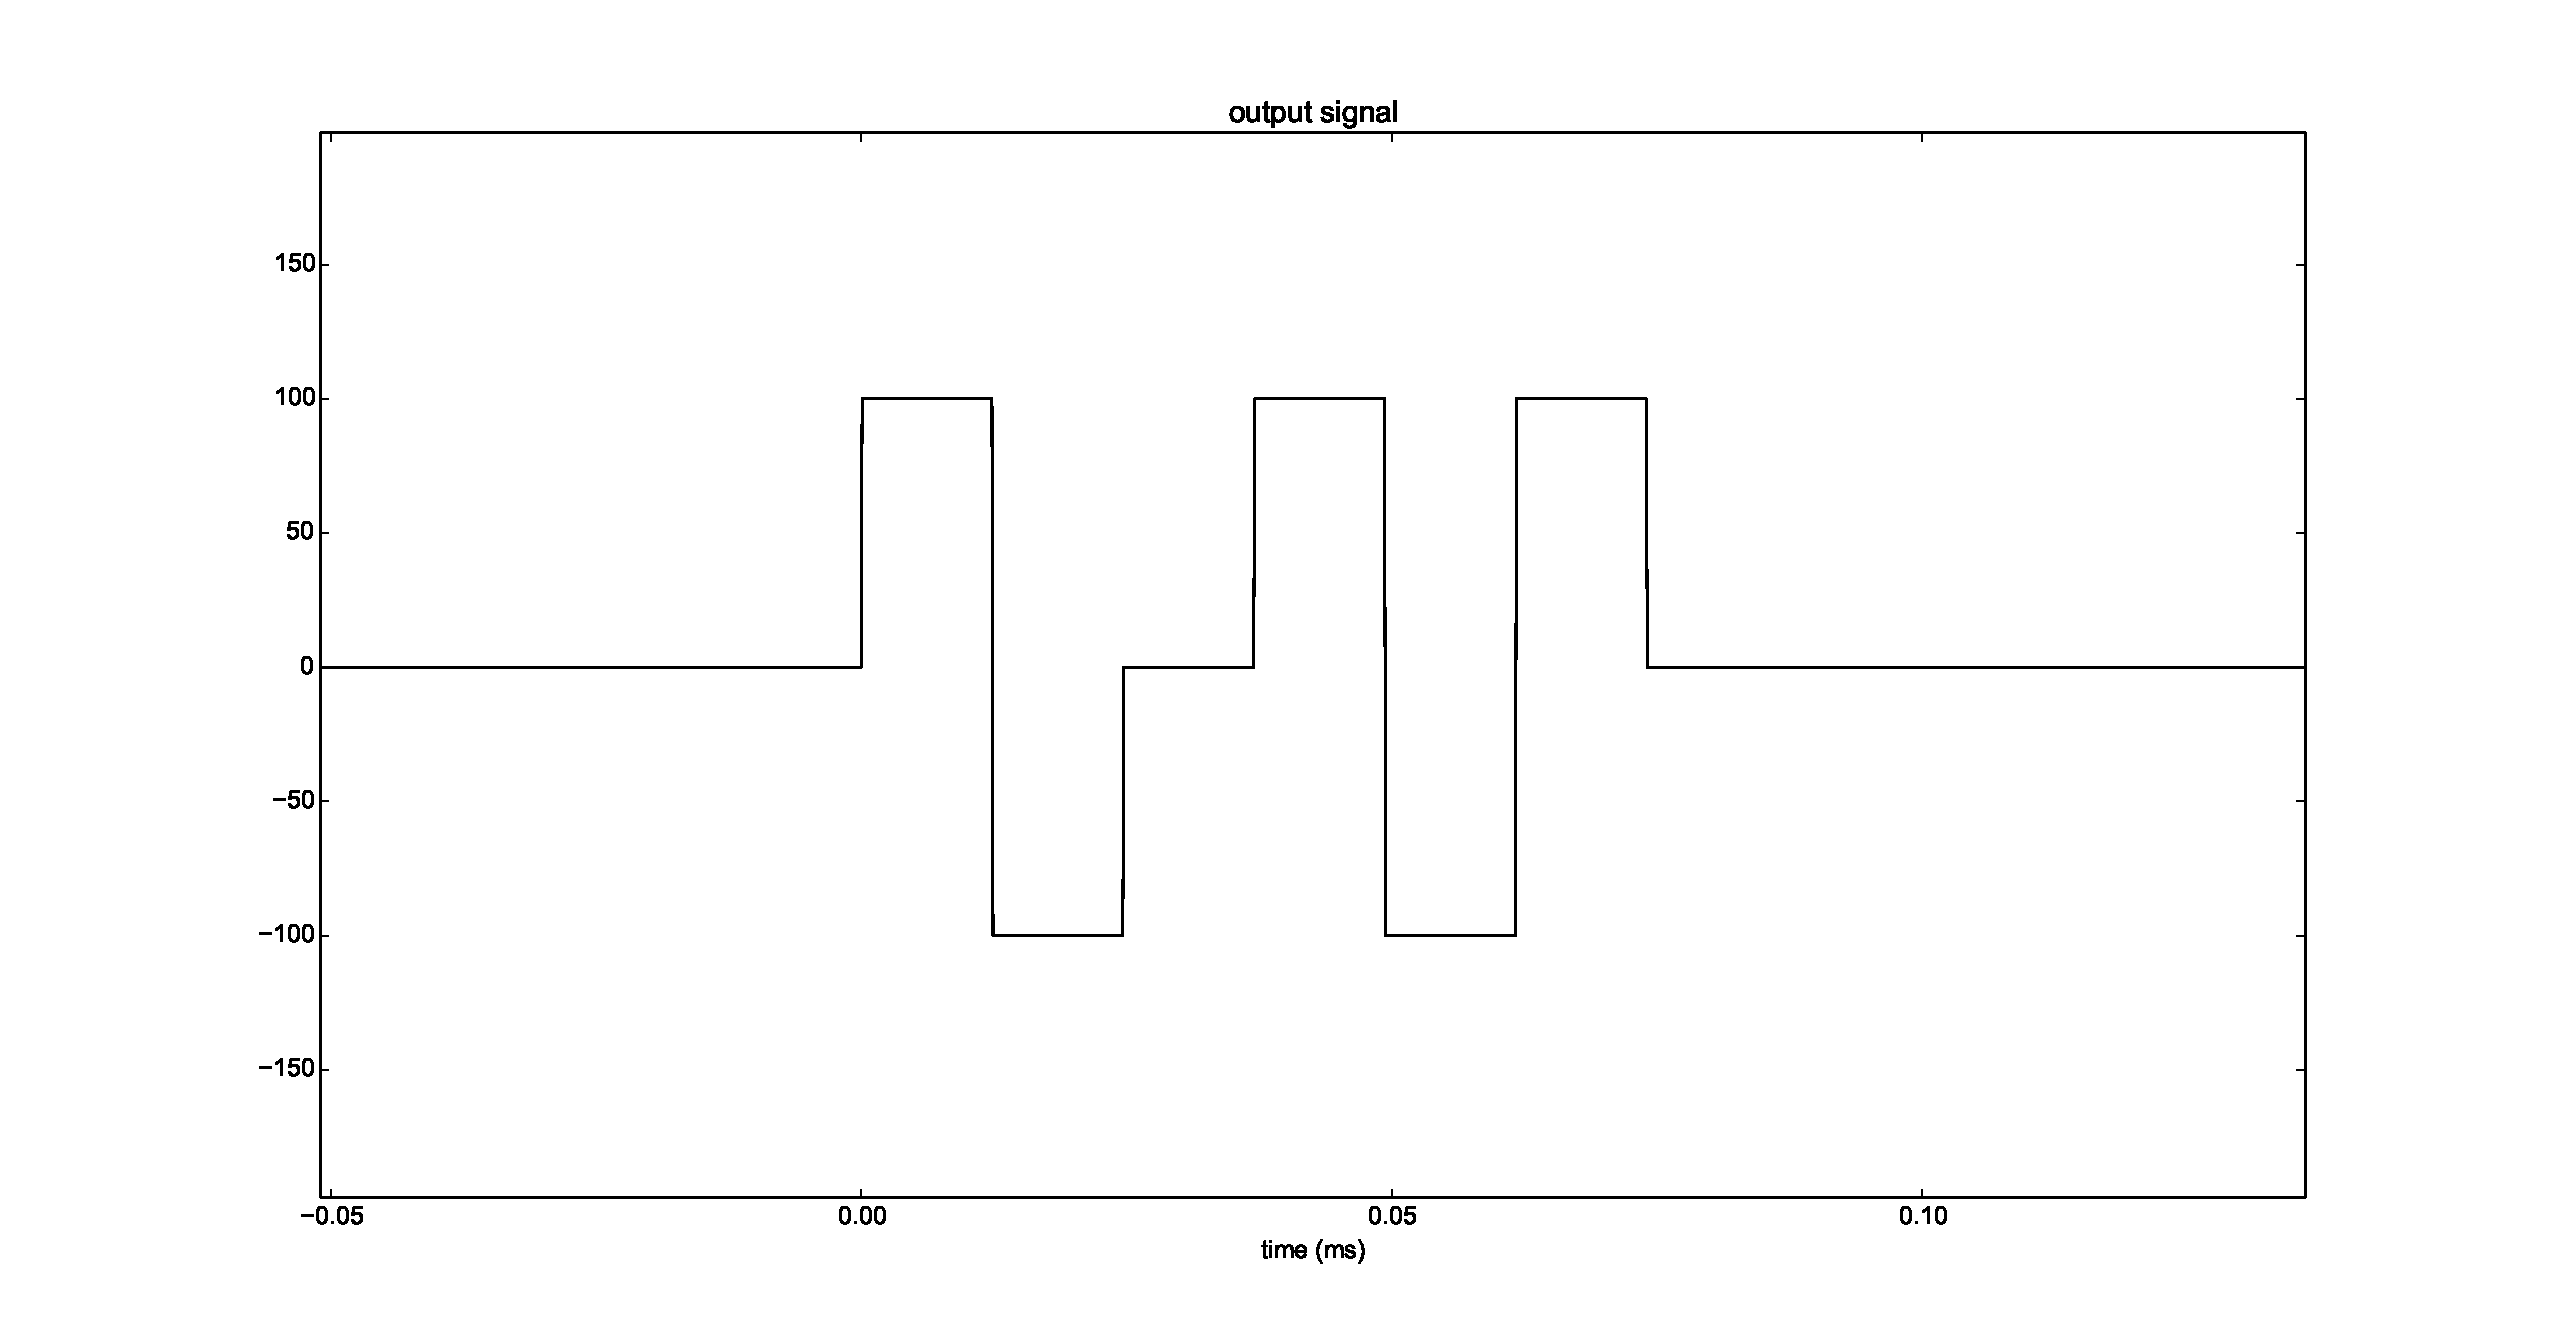
\includegraphics[width=1.15\textwidth, trim= 47mm 0mm 0mm 0mm,clip]{output_signal}
    \caption{Sygnał wysterowania nadajnika piezoelektrycznego}
    \label{fig:output_signal}
\end{figure}

\newpage

\section{Dobór rezonatorów piezoelektrycznych}

Głównym problemem podczas konstrukcji nadajnika okazał się dobór odpowiednich rezonatorów piezoelektrycznych.
Mimo, że producent wykorzystanych rezonatorów piezoelektrycznych zapewnia ich pracę zakresie: \SI{40}{kHz} $\pm$ \SI{1}{kHz}, taki rozrzut okazał się niewystarczający, 
dlatego z 30 rezonatorów (15 nadajników i 15 odbiorników) wybrane zostały 4 nadajniki i 3 odbiorniki o najbardziej 
zbliżonych częstotliwościach pracy. Częstotliwości zostały zmierzone na oscyloskopie cyfrowym, są to odpowiedzi 
rezonatora na krótki impuls elektryczny.

Tabela \ref{table:czestotliwosci} zawiera wyniki pomiarów częstotliwości, gwiazdką oznaczono wykorzystane przetworniki piezoelektryczne.

\begin{table}[t]
  \centering
  \begin{tabular}{|r|r|r|}
    \hline 
    Nr & Nadajnik: 40ST-12 & Odbiornik: 40SR-12\\
    \hline
    1  &   \SI{40,88}{kHz} & *\SI{40,65}{kHz} \\
    2  &   \SI{41,12}{kHz} &  \SI{40,45}{kHz} \\
    3  &  *\SI{40,78}{kHz} &  \SI{39,52}{kHz} \\
    4  &   \SI{41,19}{kHz} &  \SI{40,47}{kHz} \\
    5  &   \SI{40,92}{kHz} &  \SI{40,66}{kHz} \\
    6  &   \SI{39,68}{kHz} & *\SI{40,69}{kHz} \\
    7  &   \SI{39,78}{kHz} &  \SI{40,59}{kHz} \\
    8  &  *\SI{40,80}{kHz} &  \SI{40,39}{kHz} \\
    9  &   \SI{40,90}{kHz} &  \SI{40,29}{kHz} \\
    10 &  *\SI{40,66}{kHz} & *\SI{40,68}{kHz} \\
    11 &  *\SI{40,85}{kHz} &  \SI{39,22}{kHz} \\
    12 &   \SI{41,01}{kHz} &  \SI{39,51}{kHz} \\
    13 &   \SI{41,00}{kHz} &  \SI{39,92}{kHz} \\
    14 &   \SI{39,82}{kHz} &  \SI{39,26}{kHz} \\
    15 &   \SI{39,64}{kHz} &  \SI{39,11}{kHz} \\
    \hline
  \end{tabular}
  \caption{Częstotliwości rezonansowe przetworników piezoelektrycznych}
  \label{table:czestotliwosci}
\end{table}


